\documentclass[10pt]{article}
\usepackage[utf8]{inputenc}
%%%%%%%% PREÁMBULO %%%%%%%%%%%%
\usepackage[spanish,es-tabla]{babel}

\usepackage{multirow} % para las tablas
\usepackage{tcolorbox}
\tcbuselibrary{listingsutf8}
\usepackage[spanish]{babel}
\usepackage{fancybox}
\usepackage{courier}
\usepackage{ragged2e}
\usepackage[spanish]{babel}
\usepackage{amssymb, amsmath, amsbsy} % simbolitos
\usepackage{upgreek} % para poner letras griegas sin cursiva
\usepackage{cancel} % para tachar
\usepackage{mathdots} % para el comando \iddots
\usepackage{mathrsfs} % para formato de letra
\usepackage{stackrel} % para el comando \stackbin
\usepackage{courier}
\usepackage{subfig}
\usepackage{pdflscape}
\title{Plantilla Tesis MISTI ESIME}
\usepackage[spanish]{babel} %Indica que escribiermos en español
\usepackage[utf8]{inputenc} %Indica qué codificación se está usando ISO-8859-1(latin1)  o utf8  
\usepackage{amsmath} % Comandos extras para matemáticas (cajas para ecuaciones, etc)
\usepackage{amssymb} % Simbolos matematicos (por lo tanto)
\usepackage{graphicx} % Incluir imágenes en LaTeX
\usepackage{color} % Para colorear texto
%\usepackage{subfigure} % subfiguras
\usepackage{float} %Podemos usar el especificador [H] en las figuras para que se queden donde queramos
\usepackage{capt-of} % Permite usar etiquetas fuera de elementos flotantes (etiquetas de figuras)
\usepackage{sidecap} % Para poner el texto de las imágenes al lado
\sidecaptionvpos{figure}{c} % Para que el texto se alinie al centro vertical
\usepackage{caption} % Para poder quitar numeracion de figuras
\usepackage{commath} % funcionalidades extras para diferenciales, integrales, etc (\od, \dif, etc)
\usepackage{cancel} % para cancelar expresiones (\cancelto{0}{x})
\usepackage[export]{adjustbox}
\usepackage{anysize} % Para personalizar el ancho de  los márgenes
\marginsize{2cm}{2cm}{2cm}{2cm} % Izquierda, derecha, arriba, abajo

\usepackage{appendix}
\renewcommand{\appendixname}{Apéndices}
\renewcommand{\appendixtocname}{Apéndices}
\renewcommand{\appendixpagename}{Apéndices}

% Para que las referencias sean hipervínculos a las figuras o ecuaciones y aparezcan en color
\usepackage[colorlinks=true,plainpages=true,citecolor=blue,linkcolor=blue]{hyperref}
%\usepackage{hyperref}
%Para agregar encabezado y pie de página
\usepackage{fancyhdr}
\pagestyle{fancy}
\fancyhf{}
\fancyhead[L]{\footnotesize ESIME Culhuacan} %encabezado izquierda
\fancyhead[R]{\footnotesize IPN}   % dereecha
\fancyfoot[R]{\footnotesize 2024}  % Pie derecha
\fancyfoot[C]{\thepage}  % centro
\fancyfoot[L]{\footnotesize Maestría en Ingeniería en Seguridad y Tecnologías de la Información}  %izquierda
\renewcommand{\footrulewidth}{0.4pt}

\usepackage{listings} % Para usar código fuente
\definecolor{dkgreen}{rgb}{0,0.6,0} % Definimos colores para usar en el código
\definecolor{gray}{rgb}{0.5,0.5,0.5}

\newcommand{\sen}{\operatorname{\sen}}	% Definimos el comando \sen para el seno en español

\usepackage{longtable}
%%%%%%%% TERMINA PREÁMBULO %%%%%%%%%%%%

\begin{document}


\begin{center}											            							%%%
\newcommand{\HRule}{\rule{\linewidth}{0.5mm}}	                                               %%%\left
 																								%%%
\begin{minipage}{0.49\textwidth} \begin{flushleft}

\includegraphics[scale = 0.12]{Imagenes/logoesime}
\end{flushleft}\end{minipage}
\begin{minipage}{0.49\textwidth} \begin{flushright}

\includegraphics[scale = 0.25]{Imagenes/IPN}
\end{flushright}\end{minipage}

\vspace*{-1cm}			%%%

\textsc{\huge Instituto Polit\'ecnico Nacional}\\[1cm] 
\textsc{\LARGE Escuela Superior de Ingenier\'ia Mecanica y Electrica}\\[0.5cm] %%%
\textsc{\LARGE Unidad Culhuacan}\\[0.5cm] %%%
\textsc{\LARGE Ingenier\'ia en Computaci\'on }\\[1cm] %%%

\begin{minipage}{0.9\textwidth} 
\begin{center}																					%%%
\textsc{\LARGE REPORTE TÉCNICO}
\end{center}
\end{minipage}\\[0.5cm]
                                                                                    %%%
    																				%%%
 			\vspace*{1cm}															%%%
																					%%%
\HRule \\[0.1cm]																	%%%
\begin{center} \textsc{\Large Desarrollo de una plataforma para la ejecución de pruebas de carga a partir de la definición de un script con JavaScript \\}
\end{center}
\HRule \\[0.1cm]%%%
 										%%%

 																				    %%%



   \vspace{0.8cm}
\begin{center}
{\large Presenta}\\                                                                %%%
Jonathan Eduardo García García\hspace{1cm} jgarciag1404@alumno.ipn.mx
\vspace{1 cm}
\end{center}

\begin{center}
\begin{minipage}{1\textwidth}													    %%%
\begin{flushleft} \large														    %%%
\emph{Asesor del proyecto:}\\
\vspace{0.3cm}
M. en I. TIRSO MARTÍNEZ REYES\\
    \vspace*{1cm}	
                                                                %%%
\end{flushleft}	
%%%
\end{minipage}		                                            %%%
\end{center}

%\begin{minipage}{1\textwidth}													    %%%
%\begin{flushleft} \large														    %%%
%\emph{Directores del proyecto:}\\
%\vspace{0.3cm}
%M. en C. Jose Luis Cano Rosas\\
%Dr. Pedro Guevara L\'opez\

                                                                %%%
 %   \vspace*{1cm}	
                                                                %%%
%\end{flushleft}													%%%
%\end{minipage}		                                            %%%
																%%%
%\begin{flushleft}
 	
%\end{flushleft}
%%%
 		
 		            %%%
\vspace{2cm} 																				
\begin{center}
{\large \today}													%%%
\end{center}												  						

\end{center}
\cleardoublepage

\newpage
\tableofcontents

%%%%%%%%%%%%%%%%%%%%%%%%%%%%%%%%%%%%%%%%%%%%%%%%%%%%%%%%%%%%%%%%%%%%%%%%%%%%%%%%%%%%%%%
%RESUMEN
\newpage
\section{Resumen}
\justify
Esta plataforma permite la ejecución de flujos de negocio específicos para escenarios no estáticos de pruebas de carga utilizando como lenguaje principal Javascript con el cual se desarrollaron las principales funciones de la aplicación y Amazon Web Services para el almacenamiento y aprovisonamiento está, incluyendo el desarrollo un servicio API para la comunicación entre las peticiones y la base de datos.

\par\vspace{\baselineskip}
\justify
\textbf{Palabras Clave:} Pruebas de carga, Javascript, endopoint, API, multi-factor, asincrónico.

\par\vspace{\baselineskip}
%%%%%%%%%%%%%%%%%%%%%%%%%%%%%%%%%%%%%%%%%%%%%%%%%%%%%%%%%%%%%%%%%%%%%%%%%%%%%%%%%%%%%%%
%INTRODUCCIÓN 

\section{Introducción}
\justify
Las pruebas de carga para sistemas de información basados en la web se llevan a cabo de manera limitada. Tradicionalmente, estas pruebas siguen un conjunto preestablecido de peticiones dirigidas a servicios web específicos, donde los scripts de prueba dictan el flujo de ejecución. Este enfoque no permite adaptar o incluir lógicas adicionales que podrían ser necesarias para ciertos flujos de negocio específicos. Como resultado, hay ciertas restricciones en las pruebas de carga, especialmente aquellas que involucran validaciones complejas, procesamiento asincrónico y sistemas de autenticación multifactor, que no pueden ser adecuadamente evaluadas dentro del esquema de prueba convencional.
%%%%%%%%%%%%%%%%%%%%%%%%%%%%%%%%%%%%%%%%%%%%%%%%%%%%%%%%%%%%%%%%%%%%%%%%%%%%%%%%%%%%%%%
\section{Planteamiento del Problema}
\justify
Actualmente el diseño y ejecución de pruebas de carga para sistemas de información Web se basan en un flujo pre-establecido
de peticiones a un conjunto de servicios Web (endpoints) sincronizados por scripts de pruebas previamente definidos, lo cual
no deja espacio para lógica intermedia necesaria para flujos de negocio particular y por ende, limita el conjunto de flujos
de ejecución para la realización de pruebas que requieren validaciones, procesamiento asíncrono y esquemas de autenticación multi-factor.

%%%%%%%%%%%%%%%%%%%%%%%%%%%%%%%%%%%%%%%%%%%%%%%%%%%%%%%%%%%%%%%%%%%%%%%%%%%%%%%%%%%%%%%
%OBJETIVOS

\section{Objetivos}
\subsection{Objetivo General}
\justify
Implementar una plataforma que permita ejecutar scripts de pruebas de carga diseñados en JavaScript aprovechando la multitud de paquetes opensource disponibles en el registro de código (npm) y con ello extender las capacidades de las pruebas de carga a escenarios mucho más complejos, recopilando los resultados y métricas en un entorno distribuido, centralizando los resultados de la instrumentación en el tablero de control.
\\Desarrollar una interfaz (tablero de control) donde el usuario pueda ejecutar las pruebas de carga que haya diseñado y visualice las métricas de ejecución e información relevante.

\subsection{Objetivos específicos}

\begin{enumerate}
    \item Desarrollar un servicio web que cargue la definición de la prueba de carga a
          partir del código JavaScript.
    \item Desarrollar un servicio web que permita gestionar y configurar las instancias
          de cada prueba de carga durante su ejecución.
    \item Diseñar un servicio web que recupere y almacene las métricas de ejecución para
          cada prueba de carga.
    \item Diseñar una base de datos que permita almacenar la información y métricas
          relevantes a cada ejecución.
    \item Diseñar y programar una interfaz gráfica (tablero de control) que presente los
          resultados de la ejecución y la información recopilada de forma simplificada y
          unifique los resultados de cada uno de los ejecutores.
\end{enumerate}

%Límites y alcances
\section{Límites y alcances}

\begin{enumerate}
\item \textbf{Alcances.}

\begin{enumerate}
\item La plataforma soporta JavaScript como lenguaje de definición para las pruebas
de carga.
\item Adecuado para testers con conocimiento particular del flujo de la lógica de
negocio
\item Adecuado para testers con conocimiento del lenguaje JavaScript \end {enumerate}

\item  \textbf{Límites.}

\begin{enumerate}
    \item Diseñado para utilizar los servicios de AWS como aprovisionamiento
    \item El tamaño de las pruebas está limitado por la configuración especifica de la
          cuenta de AWS que se esté utilizando \end {enumerate}
\end{enumerate}

%Justificacion

\section{Justificación}
\justify
Hoy en día con el creciente aumento de necesidades de la industria en materia de ciberseguridad y pruebas de caja blanca, se requieren diseñar y ejecutar pruebas de carga de flujos de ejecución los cuales requieren integrar componentes de diversa naturaleza y origen. Quienes requieren de estas capacidades en materia de pruebas de carga optan por realizar scripts,  personalizados lo cual implica una importante inversión de tiempo y esfuerzo,  así como una limitación en la cantidad, calidad y profundidad de las métricas para evaluar el desempeño del sistema.
\\Se busca resolver con esta plataforma la falta de esta automatización y conseguir estandarizar el diseño de estas pruebas de carga.
%Estado del Arte
\section{Estado del Arte}
\justify
\cite{IEEEreferencias:Ref1} Loader.io  es un servicio de pruebas de carga gratuito que le permite realizar pruebas de esfuerzo en aplicaciones web y APIs con conexiones simultáneas.

\par\vspace{\baselineskip}
\justify
\cite{IEEEreferencias:Ref2} Herramienta de pruebas de carga de código abierto con conexiones simultáneas e implementación Cloud y local.

\par\vspace{\baselineskip}
\justify
\cite{IEEEreferencias:Ref3} Permite realizar pruebas de esfuerzo a sitios web, aplicaciones web y APIs con conexiones simultáneas desde la nube

\par\vspace{\baselineskip}
\justify
\cite{IEEEreferencias:Ref4} Herramienta de pruebas de UI con paralelización en navegadores reales.

%%%%%%%%%%%%%%%%%%%%%%%%%%%%%%%%%%%%%%%%%%%%%%%%%%%%%%%%%%%%%%%%%%%%%%%%%%%%%%%%%%%%%%%
%Marco Teórico
\section{Marco Teórico}
\subsection{Sistemas de Información}
\par\vspace{\baselineskip}
\justify
\cite{IEEEreferencias:Ref5} Los sistemas de información constituyen uno de los aspectos estratégicos claves para el buen hacer de la empresa. Para ello es necesario que la totalidad de la organización esté concienciada de su utilidad, tanto por parte de la alta dirección, la cual ha de tenerlos en cuenta a la hora de realizar el proceso de planificación estratégica de la empresa, como por parte de los distintos usuarios de la empresa. Ha de existir una política de información y motivación dentro de la empresa. Si esto se lleva a cabo, la empresa logrará superar a sus competidores, podrá aumentar su poder de negociación e incluso podrá evitar la entrada de nuevos competidores logrando la denominada “ventaja competitiva sostenible”. \par\vspace{\baselineskip}

\subsection{Pruebas de carga}
\justify
Una prueba de carga para un sistema web es un proceso que evalúa cómo el sistema se comporta al someterlo a un volumen de trabajo que replicaría un uso normal o pico de recursos por parte de los usuarios finales. Esto implica simular múltiples usuarios accediendo simultáneamente a diferentes partes del sistema web y realizando diversas operaciones para medir su rendimiento y estabilidad.\\
El objetivo principal de las pruebas de carga es identificar y diagnosticar cuellos de botella, problemas de rendimiento, y asegurarse de que el sistema puede manejar la cantidad esperada de tráfico sin deteriorarse ni fallar. Esto puede incluir comprobar la velocidad de respuesta de las páginas, la eficiencia del servidor y la base de datos bajo carga, la gestión de recursos del sistema, y la escalabilidad general de la aplicación web.\\
La prueba de carga difiere de otros tipos de pruebas, como las pruebas de estrés o pruebas de resistencia, en que no busca romper el sistema o descubrir su punto de fallo. En su lugar, trata de imitar el uso diario para garantizar que el rendimiento del sistema será adecuado cuando esté en funcionamiento y bajo la demanda de los usuarios reales.

\subsection{Base de datos}
\justify
Una base de datos es una colección organizada de información estructurada, o datos, típicamente almacenados electrónicamente en un sistema de computadora. Una base de datos es usualmente controlada por un sistema de gestión de base de datos (DBMS). En conjunto, los datos y el DBMS, junto con las aplicaciones que están asociados con ellos, se conocen como un sistema de base de datos, que a menudo se reducen a solo base de datos.
Los datos dentro de los tipos más comunes de bases de datos en funcionamiento hoy en día se modelan típicamente en filas y columnas en una serie de tablas para que el procesamiento y la consulta de datos sean eficientes. Luego se puede acceder, administrar, modificar, actualizar, controlar y organizar fácilmente los datos. La mayoría de las bases de datos utilizan lenguaje de consulta estructurado (SQL) para escribir y consultar datos. \par\vspace{\baselineskip}

\subsection{Tecnologias y software}
\begin{table}[H]
    \centering
    \par\vspace{\baselineskip}
    \begin{tabular}{| p{5 cm}| p{11cm} |}
        \hline
        Amazon Dyanmo                     & \texttt{Es una base de datos no-sql utilizada para almacenar la información, metricas y metadatos resultantes de la ejecución y configuración de las pruebas de carga. Debido a la cantidad de información que utiliza este proyecto se requiere un modelo de datos semi-estructurado para almacenar y recuperar información de forma eficiente y ordenada.} \\ \hline
        Amazon EC2                        & \texttt{Amazon Elastic Compute Cloud (Amazon EC2) proporciona capacidad de computación escalable bajo demanda en la nube, se utiliza como aprovisonamiento dinamico donde se ejecuta cada una de ka}                                                                                                                                                         \\ \hline
        Javascript                        & \texttt{Es uno de los lenguajes mas utilizados por los desarrolladores, se puede ejecutar en cualquier plataforma debido a que es interpretado y permite intregrar caracteristicas modernas para describir el flujo de las pruebas de carga.}                                                                                                                \\ \hline
        GitHub                            & \texttt{Control de versiones, en cada confirmación se especifican los cambios realizados.}                                                                                                                                                                                                                                                                   \\ \hline
        Application Programming Interface & \texttt{Se utiliza como intermediario para la comunicación entre la base de datos alojada en AWS y la aplicación. }                                                                                                                                                                                                                                          \\ \hline
        Amazon Web Services               & \texttt{Se utiliza para alojar el motor de base de datos mediante RDS , el foro de comentarios y el servicio API }                                                                                                                                                                                                                                           \\ \hline
    \end{tabular}
\end{table}
\newpage
%%%%%%%%%%%%%%%%%%%%%%%%%%%%%%%%%%%%%%%%%%%%%%%%%%%%%%%%%%%%%%%%%%%%%%%%%%%%%%%%%%%%%%%
%Metodos y Materiales
\section{Desarrollo}
\justify
Para el inicio del desarrollo del proyecto  se realizo una investigación inicial mediante un cuestionario con el cual se obtuvieron los siguientes datos cuantitativos que nos han dado una mayor viabilidad del proyecto, así como las tendencias de uso de los usuarios los cuales se muestran a continuación:

\begin{figure}[H]
    \begin{center}
        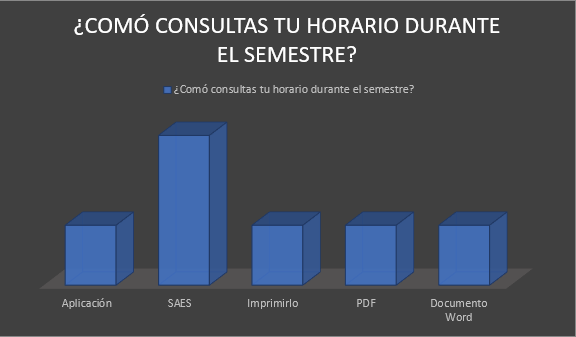
\includegraphics[width=0.7\textwidth]{Imagenes/2.PNG}
        \caption{Medios por los cuales los alumnos consultan su horario. Hemos podido observar que en su mayoría los alumnos acceden al SAES para consultar su horario, dejando otras alternativas en segundo término.}
        \label{fig16}
    \end{center}
\end{figure}
\par\vspace{\baselineskip}
\begin{figure}[H]
    \begin{center}
        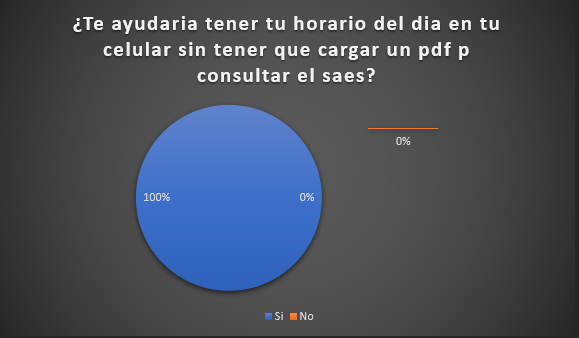
\includegraphics[width=0.7\textwidth]{Imagenes/3.PNG}
        \caption{Muestra de alumnos que preferirían tener su horario de manera más eficiente que en un PDF o consultar el saes para obtener esta información.}
        \label{fig2}
    \end{center}
\end{figure}
\par\vspace{\baselineskip}
\begin{figure}[H]
    \begin{center}
        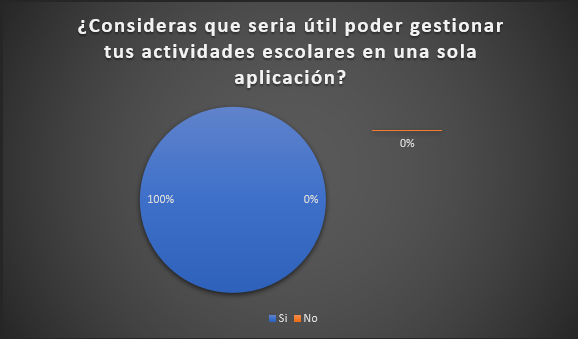
\includegraphics[width=0.7\textwidth]{Imagenes/4.PNG}
        \caption{Muestra de alumnos que preferirían gestionar en una sola aplicación todas sus actividades.}
        \label{fig3}
    \end{center}
\end{figure}
\par\vspace{\baselineskip}
\begin{figure}[H]
    \begin{center}
        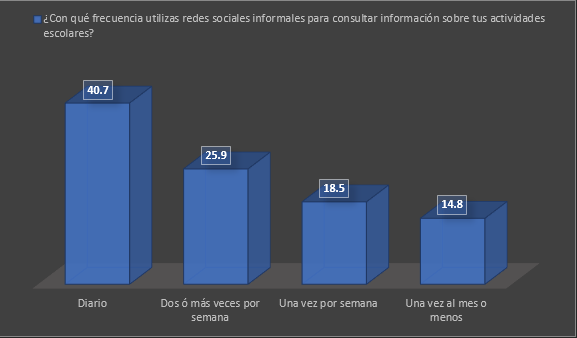
\includegraphics[width=0.7\textwidth]{Imagenes/5.PNG}
        \caption{Muestra de las veces que los alumnos visitan diversas redes sociales para obtener información de sus actividades escolares.}
        \label{fig4}
    \end{center}
\end{figure}
\par\vspace{\baselineskip}
\begin{figure}[H]
    \begin{center}
        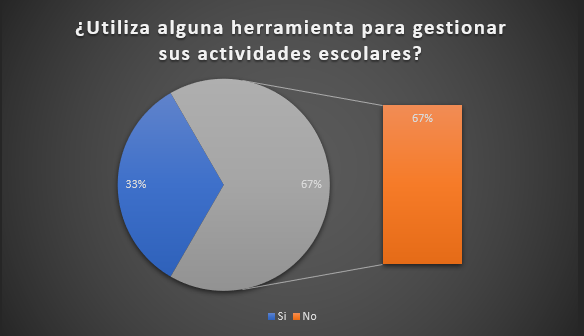
\includegraphics[width=0.7\textwidth]{Imagenes/6.PNG}
        \caption{Muestra de alumnos que sí utilizan herramientas para llevar a cabo la organización de sus actividades.}
        \label{fig5}
    \end{center}
\end{figure}
\par\vspace{\baselineskip}
\begin{figure}[H]
    \begin{center}
        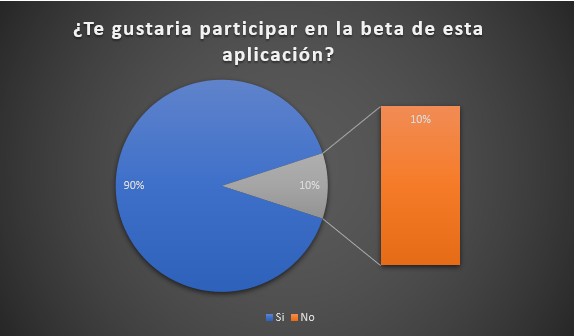
\includegraphics[width=0.7\textwidth]{Imagenes/7.PNG}
        \caption{Versión beta del Sistema. Hemos notado un interés notorio de los alumnos para probar la versión beta de la aplicación. }
        \label{fig6}
    \end{center}
\end{figure}
\par\vspace{\baselineskip}
\begin{figure}[H]
    \begin{center}
        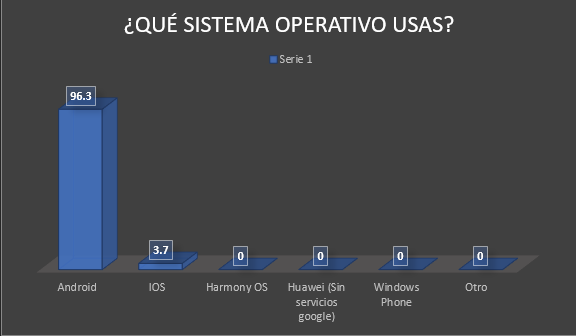
\includegraphics[width=0.7\textwidth]{Imagenes/8.PNG}
        \caption{Versiones de sistema. En esta muestra se ha observado que el 96.3\% corresponde a usuarios del Sistema Operativo Android y el 3.7\% a usuarios que utilizan IOS. }
        \label{fig7}
    \end{center}
\end{figure}

\subsection{Cronograma de actividades}
\justify
Una parte relevante del proyecto ha sido la bitácora de actividades, en ella se ven plasmados los requerimientos iniciales así como los ajustes realizados durante el desarrollo del proyecto, la bitácora nos ayudó a tener un control más adecuado de las actividades a desarrollar. Los requermientos se enlistan con la fecha en la cual se dió inicio.

\centering
\begin{table}[H]
    \begin{tabular}{|p{0.6\linewidth}|l |p{0.15\linewidth}|}
        \hline
        \textbf{Requerimiento}                                                                                               & \textbf{Fecha de inicio}  \\ \hline
        {Diseños propuestos para Login}                                                                                      & Fecha: 31/1/2021 19:30:00 \\ \hline
        {Implementación de FingerPrint}                                                                                      & Fecha: 18/2/2021 18:43:45 \\ \hline
        {Importar el horario del saes leyendo html una vez que el usuario haya iniciado sesión}                              & Fecha: 28/2/2021 21:00:26 \\ \hline
        {Pantalla de ajustes}                                                                                                & Fecha: 28/2/2021 21:01:50 \\ \hline
        {Pantalla para ver las tareas mostrando los días en los que hay actividades, al final mostrar que no hay más tareas} & Fecha: 2/6/2021 0:00:00   \\ \hline
        {Pruebsa en el acomodo de imágenes para dar de alta tareas}                                                          & Fecha: 28/2/2021 23:03:05 \\ \hline
        {Color distinto por matera}                                                                                          & Fecha: 8/3/2021 21:54:18  \\ \hline
        {Concluir ventana alta de tareas}                                                                                    & Fecha: 15/3/2021 19:02:53 \\ \hline
        {Vista de horario como tabla}                                                                                        & Fecha: 15/3/2021 19:24:27 \\ \hline
        {Recopilar nombre de las escuelas y enlaces de acceso al saes}                                                       & Fecha: 21/3/2021 21:52:35 \\ \hline
        {Obtener la información del perfil según el mockup desde el saes}                                                    & Fecha: 15/3/2021 19:25:09 \\ \hline
        {Pantalla para editar y dar de alta tareas}                                                                          & Fecha: 21/3/2021 23:24:42 \\ \hline
        {Vista de detalle por tarea}                                                                                         & Fecha: 21/3/2021 23:25:06 \\ \hline
        {Dar de alta recordatorios de exámenes ,otros eventos}                                                               & Fecha: 21/3/2021 23:29:38 \\ \hline
        {Pantalla de perfil del estudiante}                                                                                  & Fecha: 21/3/2021 23:31:08 \\ \hline
        {Exportar horario en PDF}                                                                                            & Fecha: 21/3/2021 23:43:53 \\ \hline

    \end{tabular}
\end{table}

\newpage

%%%%%%%%%%%%%%%%%%%%%%%%%%%%%%%%%%% TABLA 1 %%%%%%%%%%%%%%%%%%%%%%%%%%%%%%%%%%%%%%%%%%%%%%
\begin{table}[ht]
    \centering
    \begin{tabular}{|l |l |l |l |l |}
        \hline
        \multicolumn{3}{|c|}{\textbf{Aplicación móvil}}                                                             \\
        \hline
        \centering\textbf{Plataforma}      & {Android}                                 & {iOS}                      \\ \hline
        \centering\textbf{Versión mínima}  & {API 23+ 6.0.1 Marshmallow}               & {iOS 9}                    \\ \hline
        \centering\textbf{Versión destino} & {API 30 Honeycomb}                        & {iOS 14.5}                 \\ \hline
        \centering\textbf{Procesador}      & {arm64\-v8a, armeabi\-v7a, x86\_64}       & {A9, A10, A11, A12}        \\ \hline
        \centering\textbf{Hardware}        & {Dispositivos móviles y tabletas Android} & {Dispositivos móviles iOS} \\ \hline
    \end{tabular}
\end{table}
%%%%%%%%%%%%%%%%%%%%%%%%%%%%%%%%%%% TABLA 2 %%%%%%%%%%%%%%%%%%%%%%%%%%%%%%%%%%%%%%%%%%%%%%
\begin{table}[H]
    \begin{center}
        \begin{tabular}{| l | l |}
            \hline
            \textbf{Componente}     & \textbf{Origen}   \\ \hline
            Conectividad a internet & Requerido         \\
            Cámara                  & Deseable opcional \\ \hline
        \end{tabular}
    \end{center}
\end{table}
%%%%%%%%%%%%%%%%%%%%%%%%%%%%%%%%%%% TABLA 3 %%%%%%%%%%%%%%%%%%%%%%%%%%%%%%%%%%%%%%%%%%%%%%
\begin{table}[H]
    \centering
    \begin{tabular}{|l |l |l |l |l |}
        \hline
        \multicolumn{5}{|c|}{\textbf{Proveedor de base de datos}}                                                                                \\
        \hline
        \centering\textbf{Version SQL}                 & \textbf{CPU} & \textbf{RAM} & \textbf{Almacenamiento} & \textbf{Tipo de almacenamiento} \\ \hline
        \centering{Sqlserver express 14.00.3356.20.v1} & {1}          & {1Gb}        & {20 Gbs}                & {SSD}                           \\ \hline
        \hline
        \multicolumn{5}{|c|}{\textbf{Proveedor de servicios web}}                                                                                \\
        \hline
        \centering\textbf{Entorno}                     & \textbf{CPU} & \textbf{RAM} & \textbf{Almacenamiento} & \textbf{Tipo de almacenamiento} \\ \hline
        \centering{.NET Core 3.1 (C\#/PowerShell)}     & {1}          & {512 Mb}     & {50 Gbs}                & {SSD}                           \\ \hline
    \end{tabular}
\end{table}
\newpage
%%%%%%%%%%%%%%%%%%%%%%%%%%%%%%%%%%%%%%%%% Requerimientos funcionales 

%%%%%%%%%%%%%%%%%%%%%%%%%%%%%%%%%%%%%%%%%%%%%%%%%%%%%%%%%%%%%%%%%%%%%
\justify
\subsection{Implementacion de ISO 2000 en el proyecto}
\justify
ISO 2000
En base a la ISO 2000 se deben desarrollar los siguientes pasos:\\
\begin{itemize}
    \item Evaluar necesidades y metas de organización:\\ Se evaluaron las necesidades de
          los alumnos de la carrera de computación y la necesidad más grande fue la falta
          de organización en las tareas cotidianas escolares y la meta a desarrollo es
          una aplicación para poder administrar sus actividades escolares.
    \item Obtener información:\\ Se realizaron encuesta a los alumnos de la carrera de
          computación para saber el uso cotidiano del celular y su forma de organizar sus
          actividades escolares.
    \item Nombrar consultor:\\ Profesor Oscar Cruz García quien nos ha ayudado en la
          estructuración de las partes del proyecto.
    \item Toma de conciencia y formación:\\ a) La protección de los datos sensibles de
          los usuarios\\ b) Los objetivos de calidad pertinentes para el proyecto\\ c) La
          contribución que haremos a los alumnos y beneficios que mejoraran el desempeño
          de ellos.\\ d) Y también lo que implica incumplir los requisitos del Sistema
          proyecto.
    \item Análisis de brech:\\ Evaluamos las diferencias entre el desempeño real que
          tendrá el proyecto y el desempeño esperado que teníamos al inicio de este.
    \item Revisión o definición de procesos:\\ ¨ Se hizo un análisis de los
          requerimientos.\\ ¨ Se diagnosticaron los requerimientos funcionales y no
          funcionales.\\ ¨ Formación de las etapas de implementación de los
          requerimientos.\\ ¨ Verificación de los estándares de calidad que debe tener le
          proyecto.
    \item Suministrar personal:\\ Se organizaron las tares entre los integrantes del
          equipo para así tener un mayor desempeño en el desarrollo.\\ Establecer
          cronograma:\\ Al ya tener definidos los alcances del proyecto se implementó el
          cronograma de actividades utilizando Trello para llevar una organización de
          ellas.
\end{itemize}
\subsection{Diagrama de Casos de Uso}
\begin{figure}[H]
    \begin{center}
        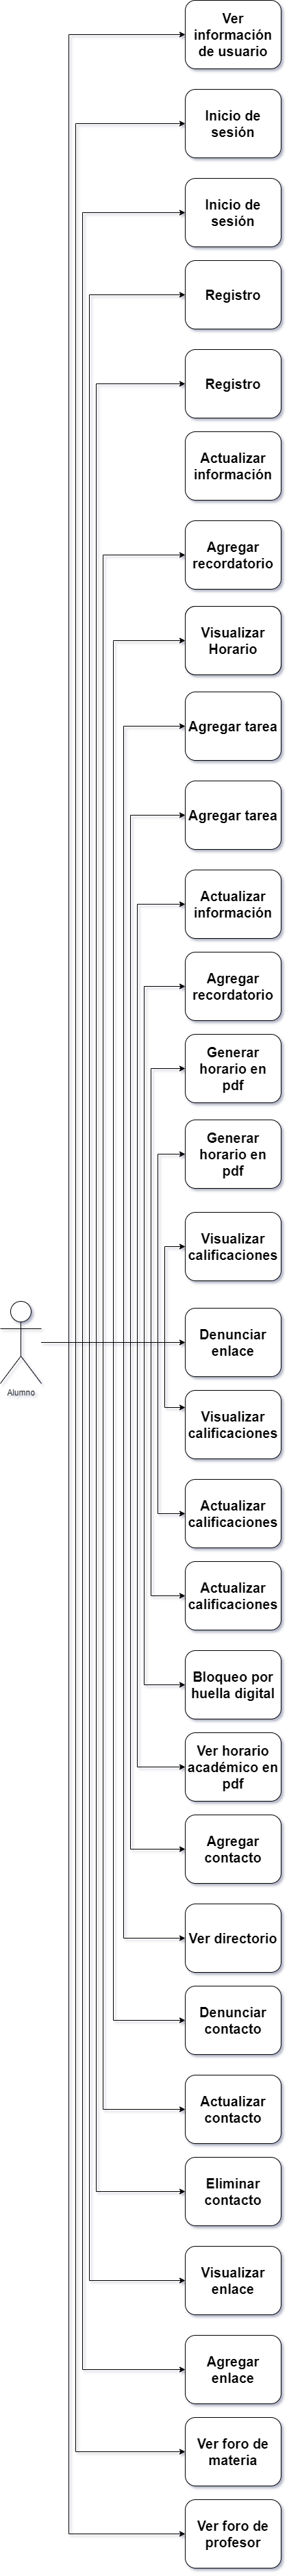
\includegraphics[width=0.13\textwidth]{Imagenes/SOE_CASOSDEUSO.PNG}
        \caption{Diagrama de casis de uso entre la aplicación y el alumno.}
        \label{fig8}
    \end{center}
\end{figure}

\newpage
\subsection{Matriz de trazabilidad de casos de uso.}

\begin{table}[ht]
    \begin{center}
        \begin{tabular}{|p{0.6\linewidth}|c |p{0.15\linewidth}|}
            \hline                                                   & Actor: Alumno \\ \hline
            {CUS1: Ver información de usuario}                       & x             \\ \hline
            {CUS2: Inicio de sesión}                                 &               \\ \hline
            {CUS3: Registro}                                         & x             \\ \hline
            {CUS4: Actualizar información}                           &               \\ \hline
            {CUS5: Agregar tarea}                                    & x             \\ \hline
            {CUS6: Agregar recordatorio}                             & x             \\ \hline
            {CUS7: Visualizar horario}                               & x             \\ \hline
            {CUS8: Generar horario en PDF}                           & x             \\ \hline
            {CUS9: Visualizar calificaciones}                        & x             \\ \hline
            {CUS10: Actualizar calificaciones}                       &               \\ \hline
            {CUS11: Activar / desactivar bloqueo por huella digital} & x             \\ \hline
            {CUS12: Activar / desactivar barra lateral de horario}   & x             \\ \hline
            {CUS13: Ver horario académico en PDF}                    & x             \\ \hline
            {CUS14: Ver directorio}                                  & x             \\ \hline
            {CUS15: Agregar contacto}                                & x             \\ \hline
            {CUS16:  Denunciar contacto}                             & x             \\ \hline
            {CUS17: Actualizar contacto}                             & x             \\ \hline
            {CUS18: Eliminar contacto}                               & x             \\ \hline
            {CUS19: Visualizar enlace}                               &               \\ \hline
            {CUS20: Agregar enlace}                                  & x             \\ \hline
            {CUS21: Denunciar enlace}                                & x             \\ \hline
            {CUS22: Ver foro de comunidad}                           & x             \\ \hline
            {CUS23: Ver foro de profesor}                            & x             \\ \hline
            {CUS24: Ver calendario escolar}                          & x             \\ \hline
            {CUS25: Mantener expandidas las tareas}                  & x             \\
            \hline
        \end{tabular}
    \end{center}
\end{table}

\justify
En donde: \\
\textbf{\\}
\textbf{CUS:} Hace referencia al caso de uso \\
\textbf{Usuario:} El actor dentro de esta matríz de trazabilidad.

\newpage
\subsection{Matriz de trazabilidad}
\noindent
\begin{longtable}{|p{0.3cm}|p{0.11\linewidth}|p{0.07\linewidth}|p{0.04\linewidth}|p{0.08\linewidth}|p{0.14\linewidth}|p{0.13\linewidth}|p{0.1\linewidth}|p{0.12\linewidth}|}
    %\begin{table}
    % \begin{tabular} {|p{0.3cm}|p{0.12\linewidth}|p{0.09\linewidth}|p{0.05\linewidth}|p{0.09\linewidth}|p{0.14\linewidth}|p{0.14\linewidth}|p{0.1\linewidth}|p{0.13\linewidth}|}
    \hline
    ID & REQUISITO                                  & TIPO         & PRIO  & ESTADO     & OBJETIVO                                                                                                                                                                                                                                & ENTREGABLE                                  & ESTADO     & VALIDACIÓN               \\ \hline
    1  & Protección   biométrica                    & Android/ IOS & Alta  & Finalizado & Uso del sistema biométrico por huella para   protección de la aplicación.                                                                                                                                                               & Desbloqueo   de la aplicación con biometría & Testing    & 17 de ago. a las 20:05   \\ \hline
    2  & Visualizar horario                         & Saes         & Alta  & Finalizado & Visualización de horario actual ordenado por   clase y colores                                                                                                                                                                          & Horario Obtenido del saes                   & Completado & 28 de mar. a las 22:59   \\ \hline
    3  & Exportar horario en PDF                    & Research     & Media & Finalizado & Generar el horario en formato PDF                                                                                                                                                                                                       & Se obtiene una versión en PDF del horario   & Completado & 6 de abr. a las 20:28    \\ \hline
    4  & Pantalla   de perfil del estudiante        & Diseño       & Alta  & Finalizado & Al ingresar por primera vez se   podrá visualizar la información del alumno como carrera, escuela y avance   escolar                                                                                                                    & Venta perfil de estudiante                  & Completado & 17 de ago. a las 20:04   \\ \hline
    5  & Widget   de horario                        & Android      & Alta  & Finalizado & Desarrollo de widget de horario   orientado a Android                                                                                                                                                                                   & Widget de horario [Android]                 & Completado & 08 de jun. a   las 00:00 \\ \hline
    6  & Esquema   de servidor                      & API          & Alta  & Finalizado & Una iniciativa para eliminar el procesamiento   en el dispositivo de cliente y apostar por una arquitectura más segura                                                                                                                  & API                                         & Completado & 01 de jul. a las 00:00   \\ \hline
    7  & Crea   recordatorios                       & Page         & Alta  & Finalizado & Creación de recordatorios por   materia con título, descripción, fecha de inicio y fin                                                                                                                                                  & Lamba AWS Cloud clusters                    & Completado & 17 de ago. a las 20:04   \\ \hline
    8  & Crea   tareas                              & Page         & Alta  & Finalizado & Creación de tareas por materia con   título, descripción, fecha de inicio y fin, así como adjuntar imágenes                                                                                                                             & Ventana de altas                            & Testing    & 17 de ago. a las 20:05   \\ \hline
    9  & Consulta   calificaciones                  & Saes         & Alta  & Finalizado & Visualizar las calificaciones y   actualizar las mismas                                                                                                                                                                                 & Ventana de calificaciones                   & Testing    & 17 de ago. a las 20:05   \\ \hline
    10 & Widget de tareas [Android]                 & Android      & Alta  & Finalizado & Desarrollo de widget de tareas   orientado a Android                                                                                                                                                                                    & Widget de tareas [Android]                  & Testing    & 17 de ago. a   las 20:05 \\ \hline
    11 & Compartir   Tarea                          & API/ Diseño  & Alta  & Finalizado & Se pueden adjuntar enlaces de   interés para un grupo de clase                                                                                                                                                                          & Compartir   enlaces                         & Testing    & 17 de ago. a las 20:05   \\ \hline
    13 & Notificaciones   10 minutos antes de clase & Research     & Alta  & Finalizado & Función para compartir las tareas                                                                                                                                                                                                       & Compartir tarea                             & Testing    & 17 de ago. a las 20:05   \\ \hline
    12 & Compartir   enlaces                        & API/ Diseño  & Alta  & Finalizado & Recibe notificaciones 10 minutos   previos al inicio de cada clase                                                                                                                                                                      & Recordatorios 10 minutos                    & Testing    & 17 de ago.   a las 20:05 \\ \hline
    14 & Notificaciones   de tarea                  & Research     & Alta  & Finalizado & Recibe notificaciones de tareas   próximas a vencer                                                                                                                                                                                     & Recordatorios por tarea                     & Testing    & 17 de ago. a las 20:05   \\ \hline
    15 & Adjuntar   imágenes en tareas              & Page         & Alta  & Finalizado & Al crear una tarea se pueden   adjuntar imágenes desde la galería o cámara fotográfica                                                                                                                                                  & Actualización ventana de altas              & Testing    & 17 de ago.   a las 20:05 \\ \hline
    16 & Información por materia                    & Page         & Alta  & Finalizado & Se desplegará información relevante   sobre la materia como el grupo y la clase a tomar, así como un foro para estudiantes   para discutir temas de la clase así cómo saber qué alumnos están inscritos en   ella (compañeros de clase) & Actualización ventana de altas              & Testing    & 17 de ago. a las 20:05   \\ \hline
    17 & Muro   de tareas y recordatorios           & Page         & Alta  & Finalizado & La pantalla principal muestra las   tareas y recordatorios ordenados por orden de importancia (fecha a expirar)                                                                                                                         & Actualización ventana de altas              & Testing    & 17 de ago.   a las 20:05 \\ \hline
\end{longtable}
%\end{table}

\subsection{Diagrama de funcionamiento}
\begin{figure}[H]
    \begin{center}
        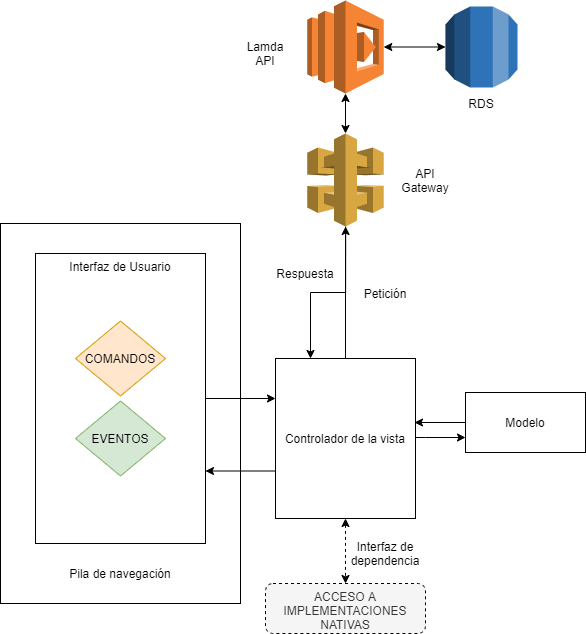
\includegraphics[width=1\textwidth]{Imagenes/11.PNG}
        \caption{Funcionamiento general de la aplicación y su comunicación con la nube.}
        \label{fig9}
    \end{center}
\end{figure}
\subsection{Modelo de  solución de software}
\begin{figure}[H]
    \begin{center}
        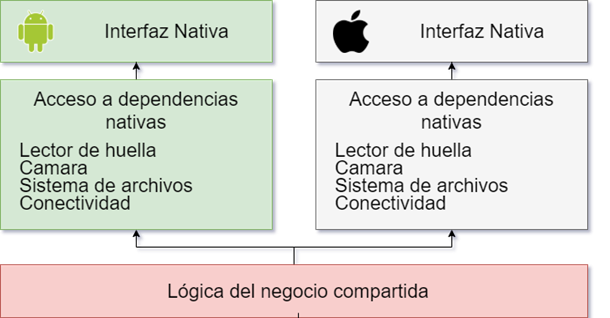
\includegraphics[width=0.8\textwidth]{Imagenes/12.PNG}
        \caption{Modelo de arquitectura interna de la solución multiplataforma.}
        \label{fig11}
    \end{center}
\end{figure}

\subsection{Diagrama de funcionamiento ventana principal}
\begin{figure}[H]
    \begin{center}
        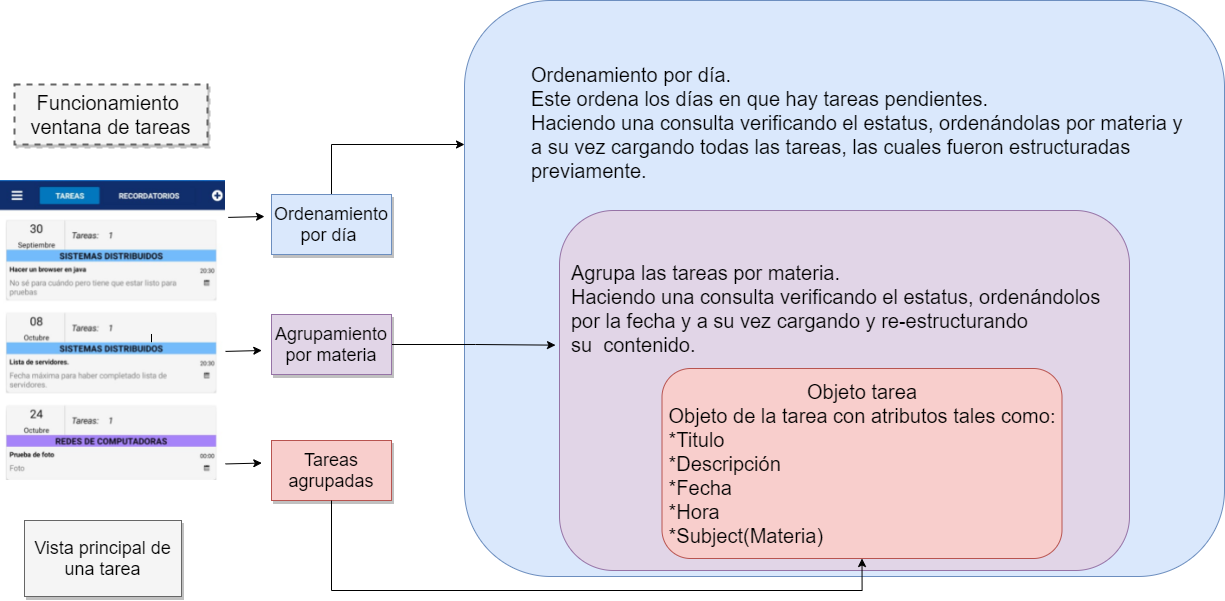
\includegraphics[width=0.8\textwidth]{Imagenes/DiagramaTareas.png}
        \caption{Esquema de la estructura de la ventana de tareas}
        \label{fig12}
    \end{center}
\end{figure}
\begin{landscape}
    \subsection{Diagrama entidad-relación}
    \begin{figure}[h]
        \centering
        \begin{center}
            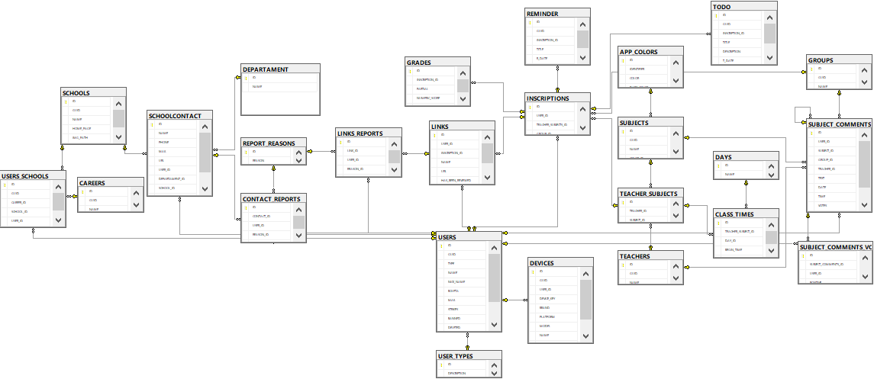
\includegraphics[width=1.3\textwidth]{Imagenes/diagrama.png}
            \caption{Diagrama entidad-relación de la base de datos alojada en el servicio web.}
            \label{fig13}
        \end{center}
    \end{figure}
\end{landscape}
\newpage
\subsection{Desarrollo de API}
\begin{figure}[H]
    \begin{center}
        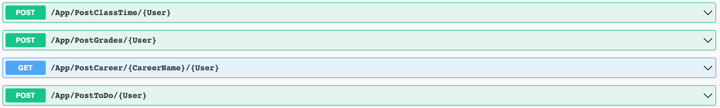
\includegraphics[width=0.8\textwidth]{Imagenes/api.png}
        \caption{Ejemplos de verbos modificadores y recuperadores de el API}
        \label{4}
    \end{center}
\end{figure}
\begin{figure}[H]
    \begin{center}
        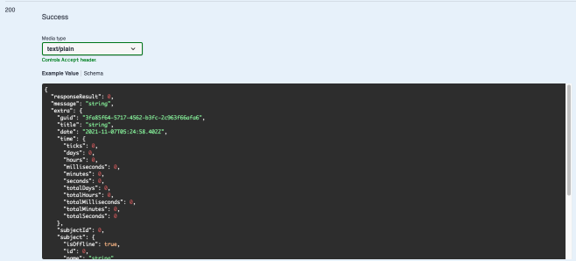
\includegraphics[width=0.8\textwidth]{Imagenes/api2.png}
        \caption{Ejemplo de respuesta del verbo modificador "ShareTodo"}
        \label{fig15}
    \end{center}
\end{figure}
\subsection{Llamada desde la aplicación al API}
\begin{figure}[H]
    \begin{center}
        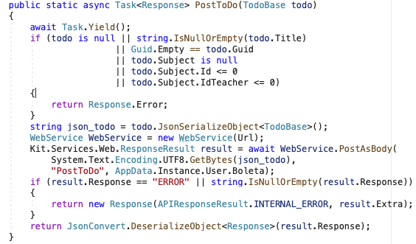
\includegraphics[width=0.8\textwidth]{Imagenes/api3.png}
        \caption{Fragmento de código de la llamada desde la aplicación a el servicio Web}
        \label{fig17}
    \end{center}
\end{figure}
\begin{figure}[H]
    \begin{center}
        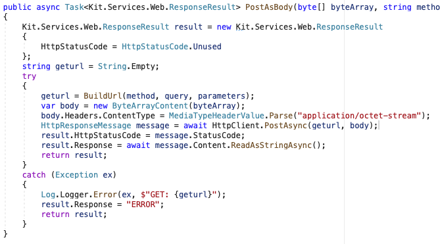
\includegraphics[width=0.8\textwidth]{Imagenes/api4.png}
        \caption{Fragmento de código de las llamada POST}
        \label{fig18}
    \end{center}
\end{figure}
\subsection{Fragmento de código de la pantalla para dar de alta una tarea}
\begin{figure}[H]
    \begin{center}
        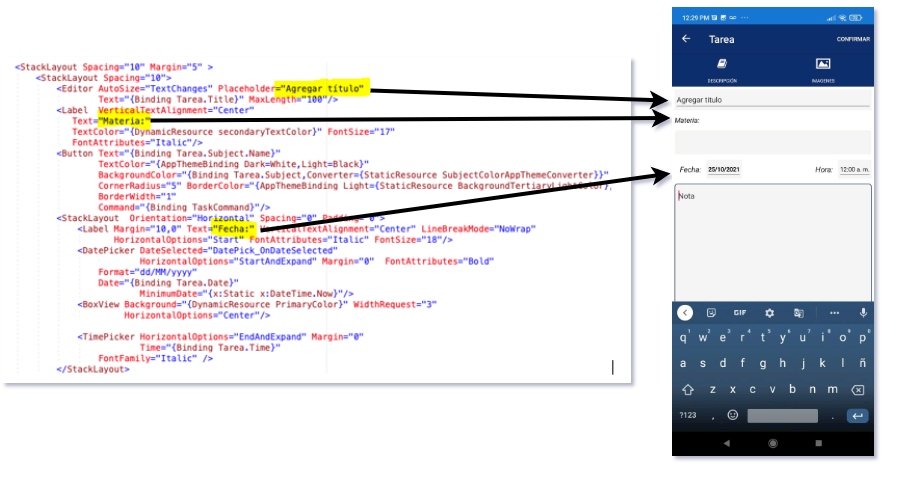
\includegraphics[width=1\textwidth]{Imagenes/tareas.png}
        \caption{Fragmento de código del maquetado de la interfaz gráfica en la pantalla para dar de alta una tarea}
        \label{fig19}
    \end{center}
\end{figure}

\subsection{Implementación widget nativo}
\begin{figure}[H]
    \begin{center}
        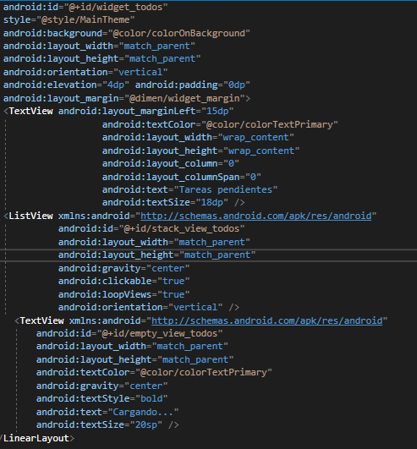
\includegraphics[width=0.8\textwidth]{Imagenes/widget.png}
        \caption{Fragmento de código de la interfaz gráfica del widget nativo para Android.}
        \label{fig1}
    \end{center}
\end{figure}
\begin{figure}[H]
    \centering
    \subfloat[\centering Widget de tareas]{{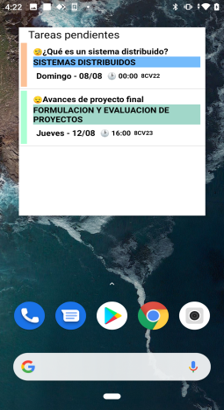
\includegraphics[height=12cm]{Imagenes/widget1} }}%
    \qquad
    \subfloat[\centering Widget de horario]{{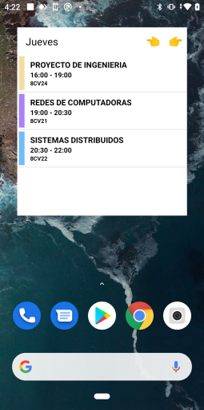
\includegraphics[height=12cm]{Imagenes/widget2} }}%
    \caption{Widget nativo (Andorid)}%
    \label{fig:example}%
\end{figure}
\newpage

\subsection{Principales funcionalidades de la aplicación.}
\begin{figure}[ht!]% 
    \begin{minipage}[b]{0.49\linewidth}%
        \centering
        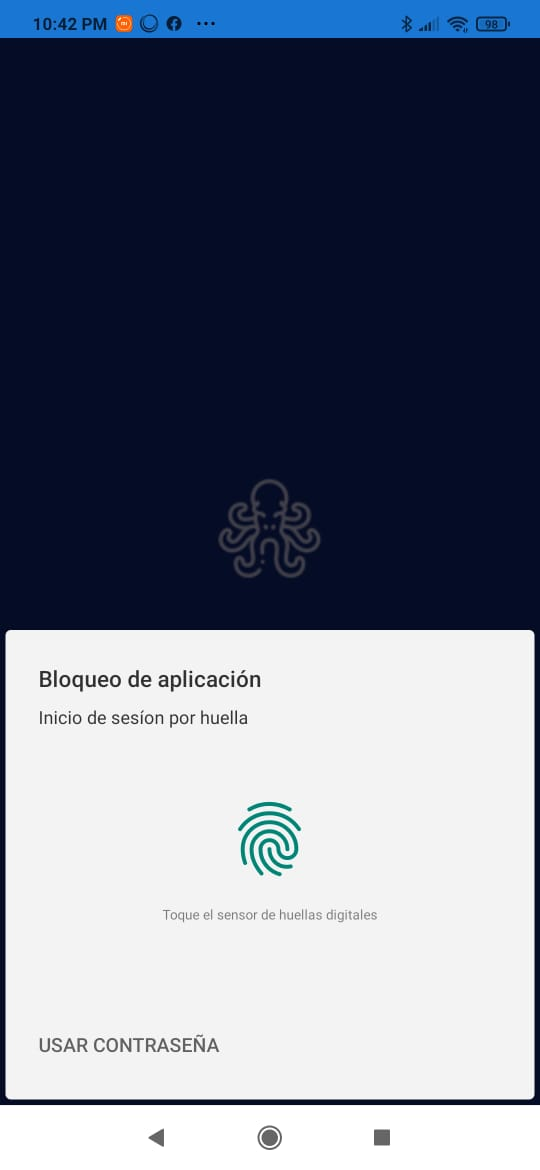
\includegraphics[width=.4\linewidth]{Imagenes/SOE1.jpeg} %
        \caption{En el inicio de sesión se despliega la \\ opción para ingresar por medio de huella,\\ alternativamente por contraseña.}%
    \end{minipage}%%
    \vspace{1cm}%
    \begin{minipage}[b]{0.49\linewidth}
        \centering
        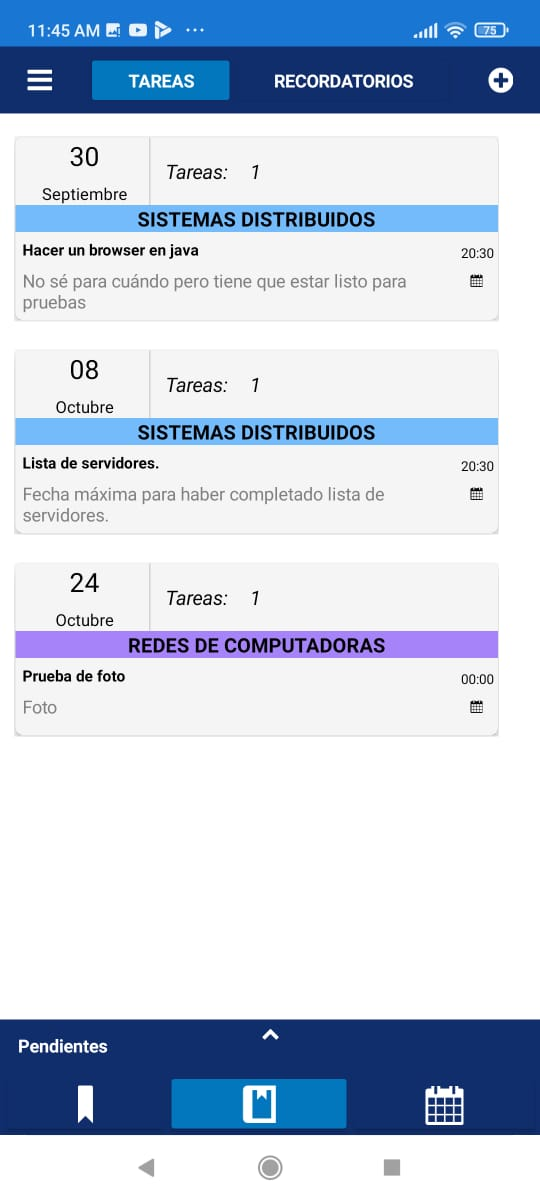
\includegraphics[width=.4\linewidth]{Imagenes/SOE2.jpeg}
        \caption{La pantalla de tareas es la primera en mostrarse una vez que se ingresa a la aplicación.}
    \end{minipage} %
    \vspace{1cm}%
    \begin{minipage}[b]{0.49\linewidth}
        \centering
        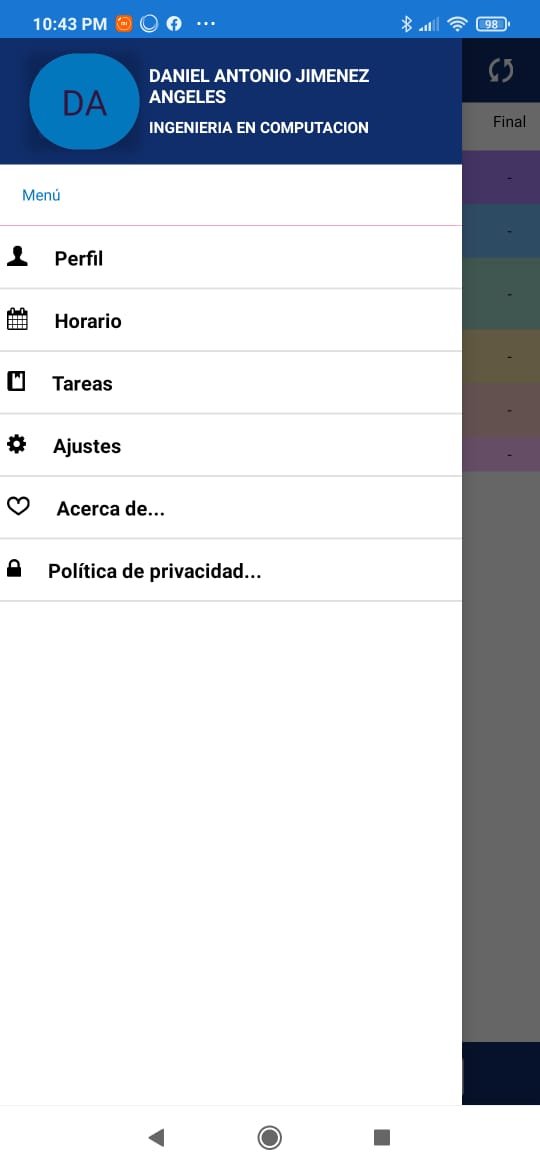
\includegraphics[width=.4\linewidth]{Imagenes/SOE3.jpeg}
        \caption{En esta pantalla de muestran los\\ siguientes submenús: Perfil, horario, tareas,\\ ajustes, aderca de y política de privacidad.}
    \end{minipage}%% 
    \vspace{1cm}%
    \begin{minipage}[b]{0.49\linewidth}%
        \centering%
        
\includegraphics[width=.4\linewidth]{Imagenes/SOE4.jpeg} %
        \caption{Ingresando a la opción perfil
            se muestran datos del alumno: Nombre, Escuela, Boleta, Carrea, Semestre, Créditos totales, Créditos obtenidos, Créditos aprobados*.}%
    \end{minipage}% 
    \vspace{1cm}%
\end{figure}%
%
\newpage

\begin{figure}[ht!]
    \begin{minipage}[b]{0.49\linewidth}
        \centering
        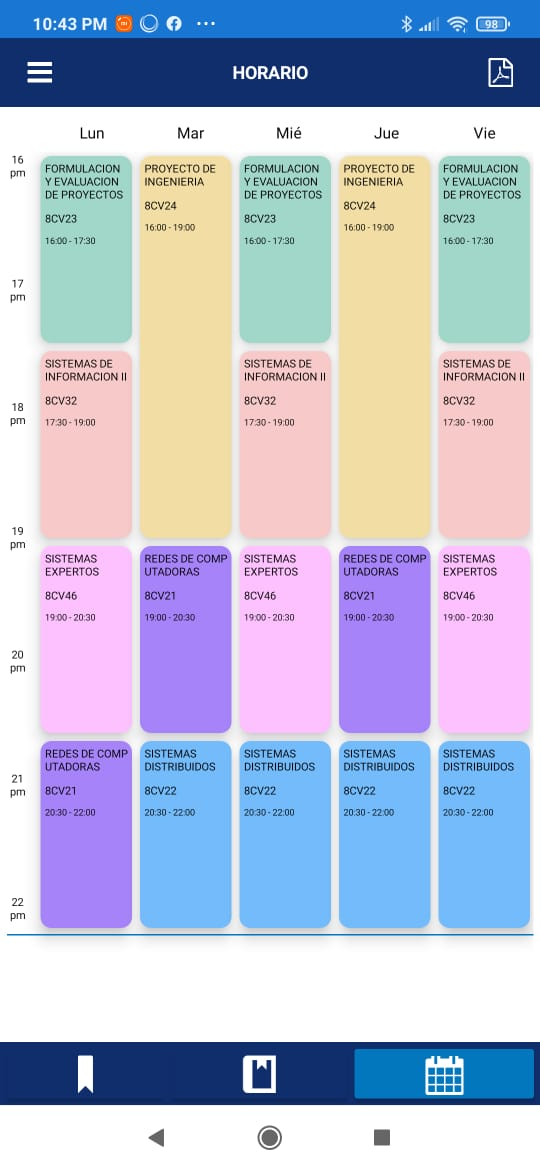
\includegraphics[width=.4\linewidth]{Imagenes/SOE5.jpeg}
        \caption{En el inicio de sesión se despliega la \\ opción para ingresar por medio de huella,\\ alternativamente por contraseña.}
    \end{minipage}%%
    \vspace{1cm}
    \begin{minipage}[b]{0.49\linewidth}
        \centering
        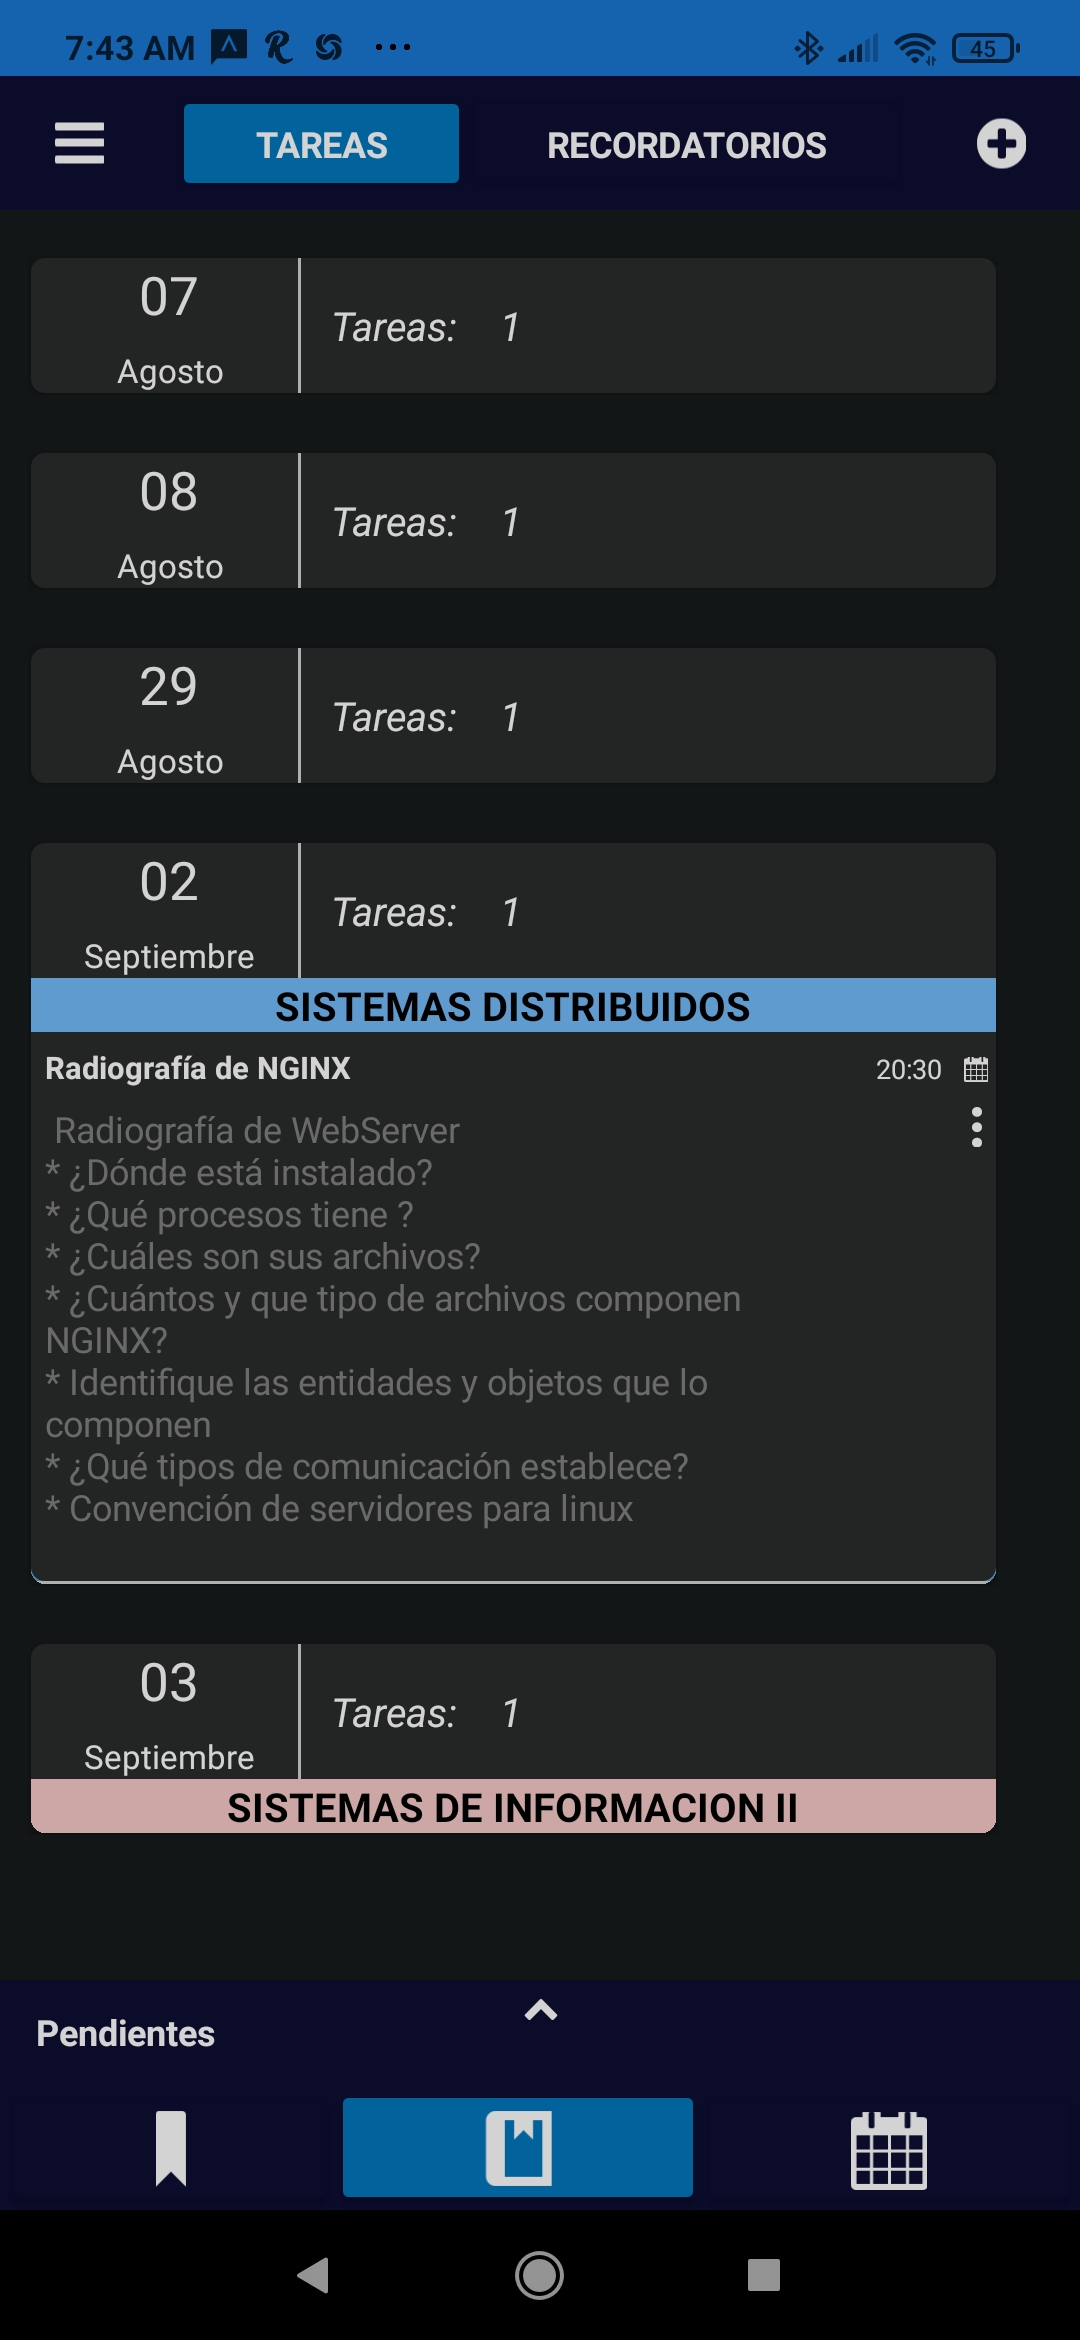
\includegraphics[width=.4\linewidth]{Imagenes/SOE6.jpg}
        \caption{La pantalla de tareas es la primera en mostrarse una vez que se ingresa a la aplicación.}
    \end{minipage}
    \vspace{1cm}
    \begin{minipage}[b]{0.49\linewidth}
        \centering
        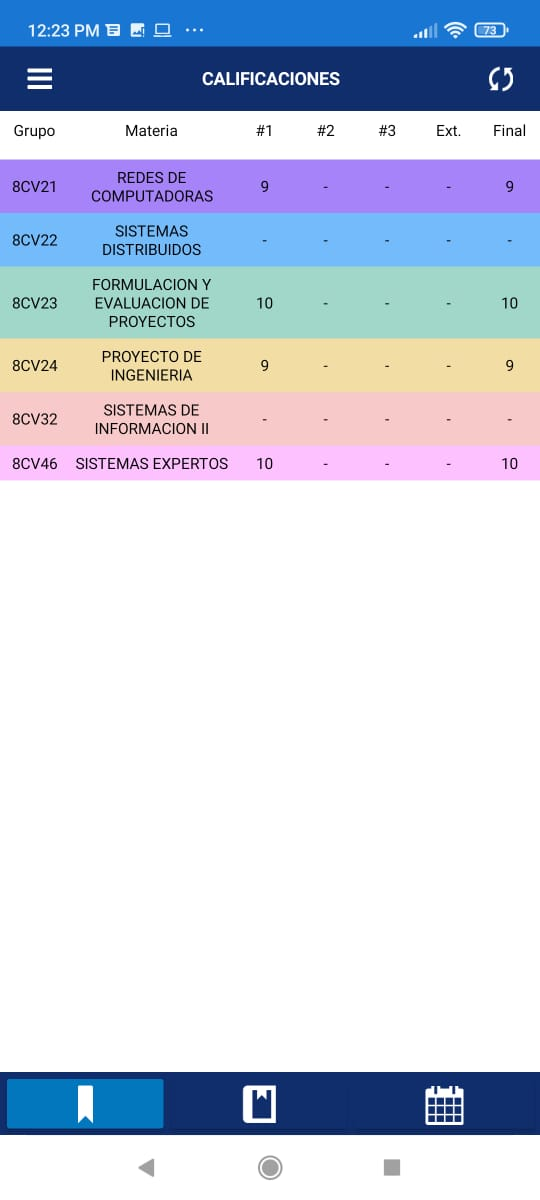
\includegraphics[width=.4\linewidth]{Imagenes/SOE7.jpeg}
        \caption{En esta pantalla de muestran los\\ siguientes submenús: Perfil, horario, tareas,\\ ajustes, aderca de y política de privacidad.}
    \end{minipage}%% 
    \vspace{1cm}
    \begin{minipage}[b]{0.49\linewidth}
        \centering
        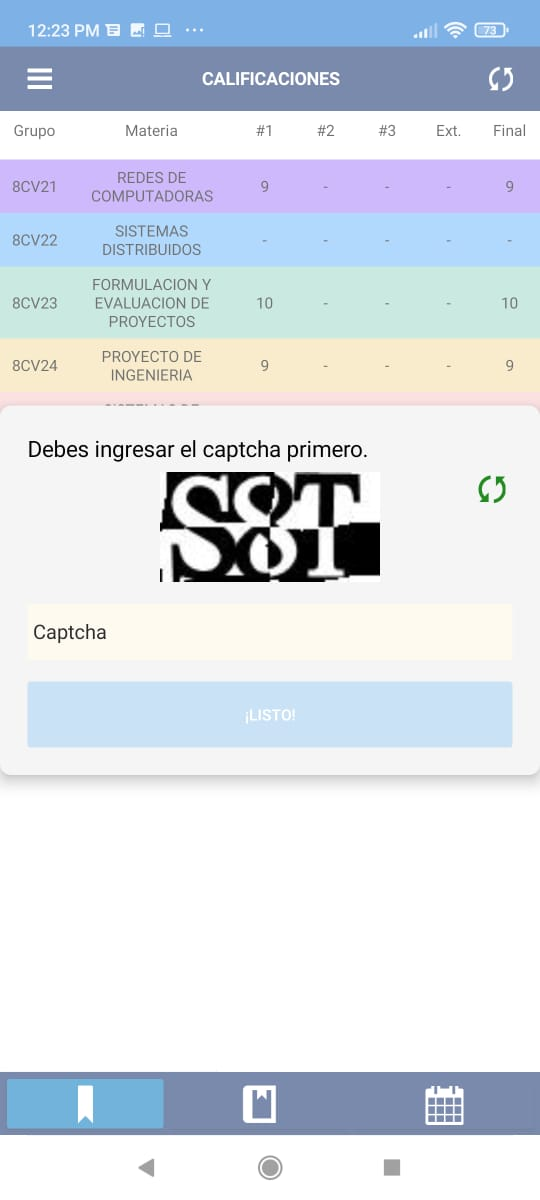
\includegraphics[width=.4\linewidth]{Imagenes/SOE8.jpeg}
        \caption{Ingresando a la opción perfil
            se muestran datos del alumno: Nombre, Escuela, Boleta, Carrea, Semestre, Créditos totales, Créditos obtenidos, Créditos aprobados*.}
    \end{minipage}
    \vspace{1cm}
\end{figure}

\newpage

\begin{figure}[ht!]
    \begin{minipage}[b]{0.49\linewidth}
        \centering
        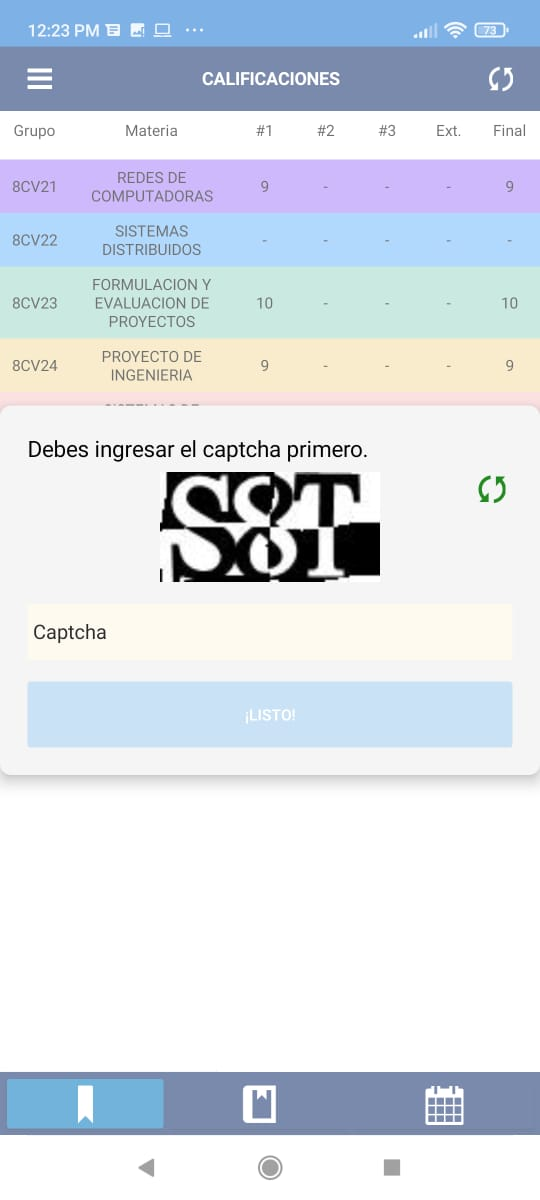
\includegraphics[width=.4\linewidth]{Imagenes/SOE8.jpeg}
        \caption{Una vez resuelto el captcha\\ las calificaciones se actualizan en automático.}
    \end{minipage}%%
    \vspace{1cm}
    \begin{minipage}[b]{0.49\linewidth}
        \centering
        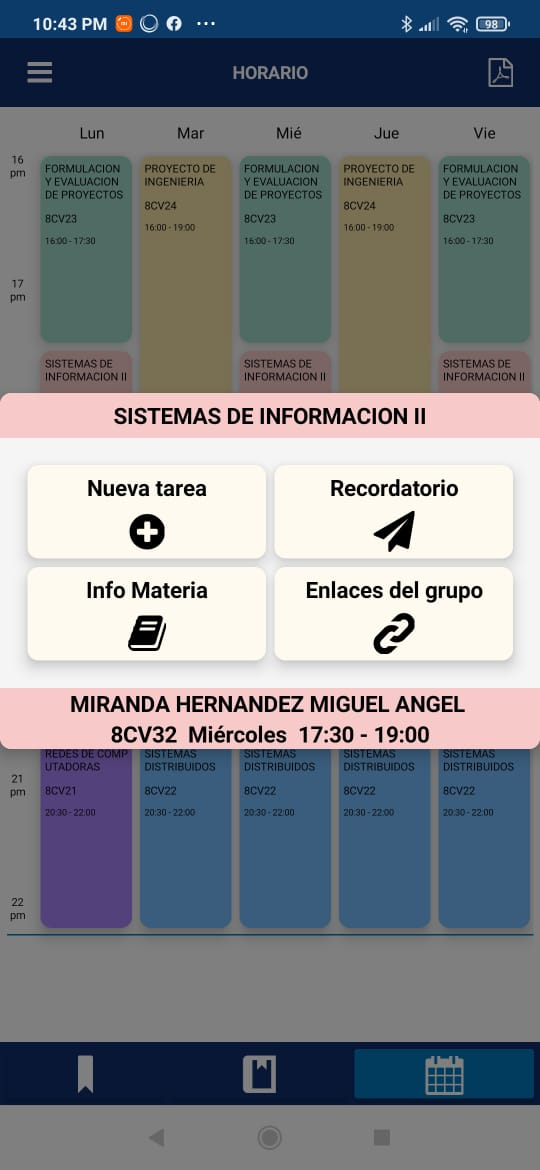
\includegraphics[width=.4\linewidth]{Imagenes/SOE9.jpeg}
        \caption{La pantalla de horario muestra las clases inscritas con dos ejes de referencia; los días de la semana de lunes a viernes y un rango de horas desde el inicio hasta el fin de clases en el día.}
    \end{minipage}
    \vspace{1cm}
    \begin{minipage}[b]{0.49\linewidth}
        \centering
        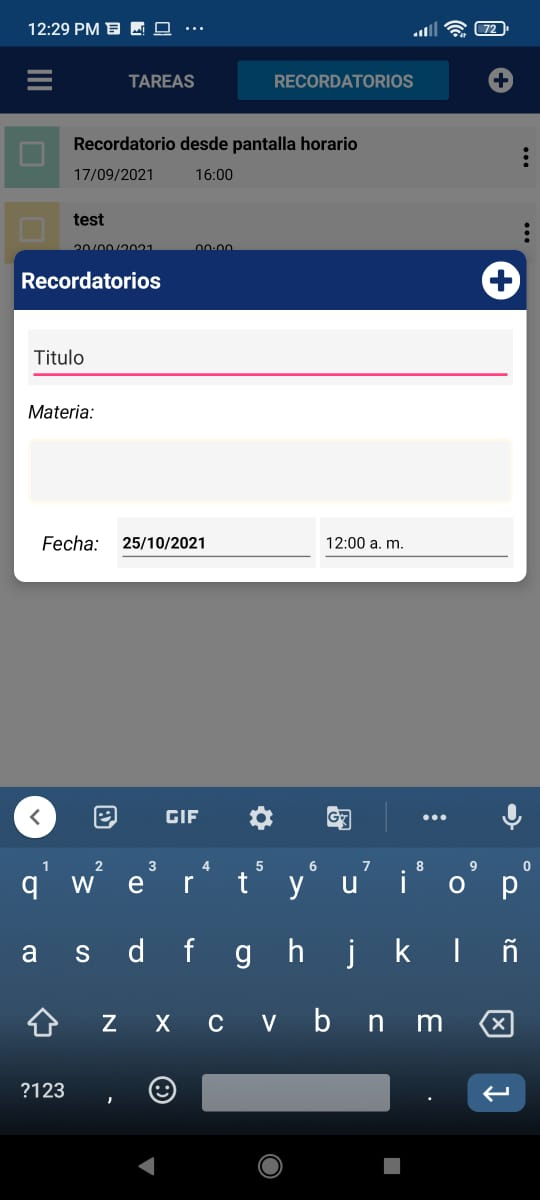
\includegraphics[width=.4\linewidth]{Imagenes/SOE10.jpeg}
        \caption{En la opción recordatorio tenemos\\ cuatro campos para editar: Título, Materia,\\ Fecha de entrega,Hora de entrega}
    \end{minipage}%% 
    \vspace{1cm}
    \begin{minipage}[b]{0.49\linewidth}
        \centering
        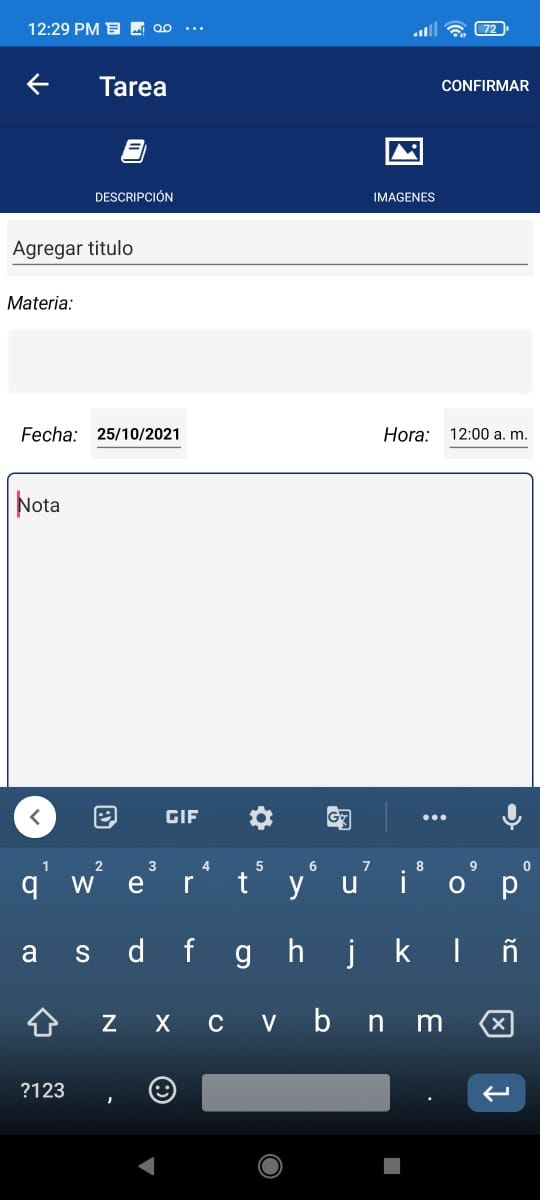
\includegraphics[width=.4\linewidth]{Imagenes/SOE11.jpeg}
        \caption{En la opción tarea tenemos cuatro campos para editar: Título, Nota, Fecha de entrega, Hora de entrega, Imágenes}
    \end{minipage}
    \vspace{1cm}
\end{figure}

\newpage

\begin{figure}[ht!]
    \begin{minipage}[b]{0.49\linewidth}
        \centering
        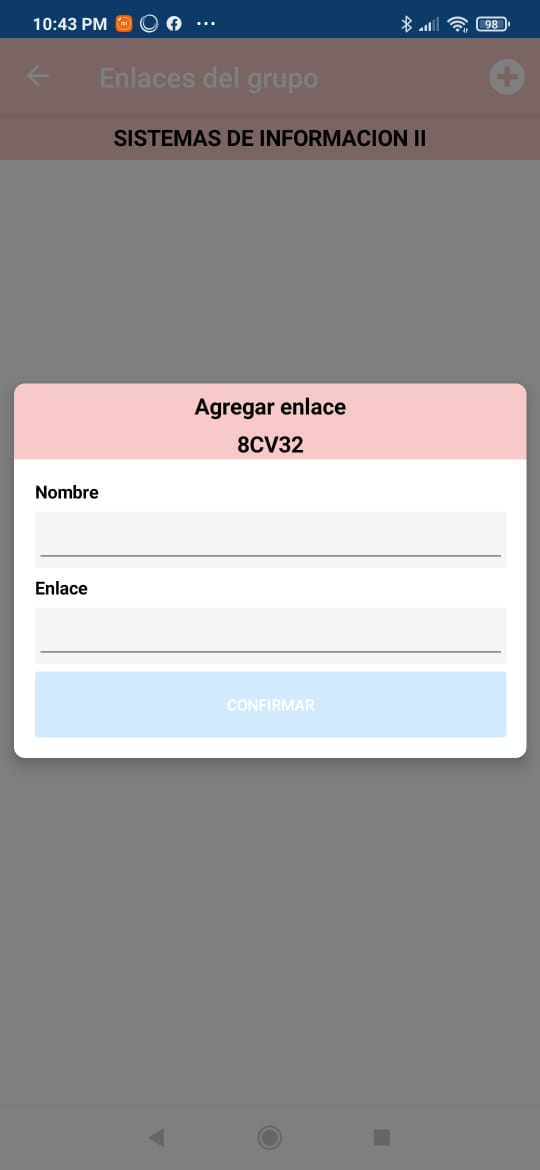
\includegraphics[width=.4\linewidth]{Imagenes/SOE13.jpeg}
        \caption{Tenemos la opción de agregar un\\ enlace en la clase seleccionada como por\\ ejemplo una reunión en alguna plataforma.}
    \end{minipage}%%
    \vspace{1cm}
    \begin{minipage}[b]{0.49\linewidth}
        \centering
        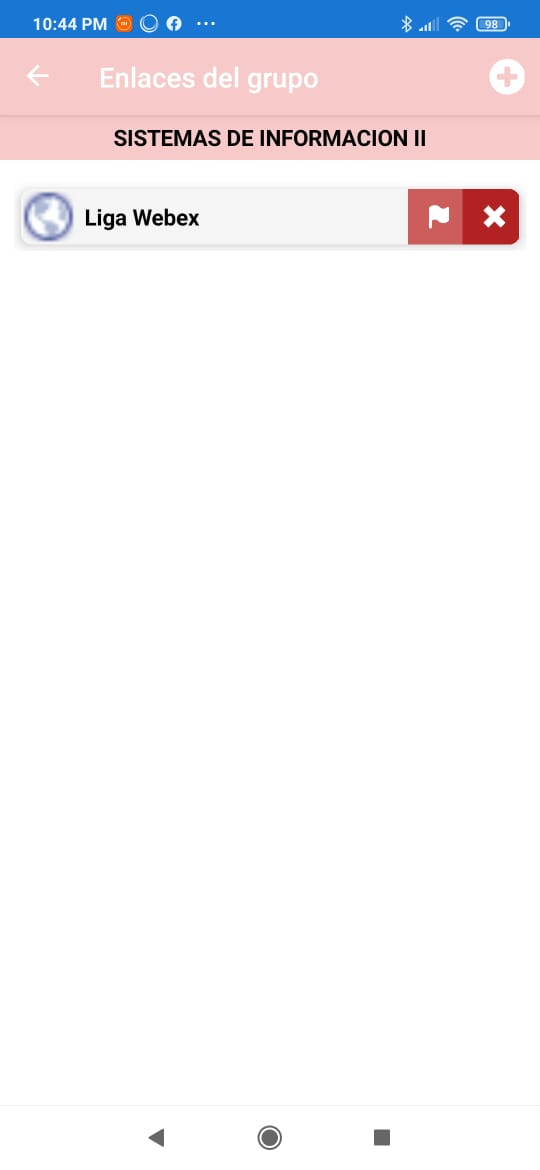
\includegraphics[width=.4\linewidth]{Imagenes/SOE14.jpeg}
        \caption{Vista del enlace una vez creado, cualquier ususario puede ingresar a él presionando sobre el mismo.}
    \end{minipage}
    \vspace{1cm}
    \begin{minipage}[b]{0.49\linewidth}
        \centering
        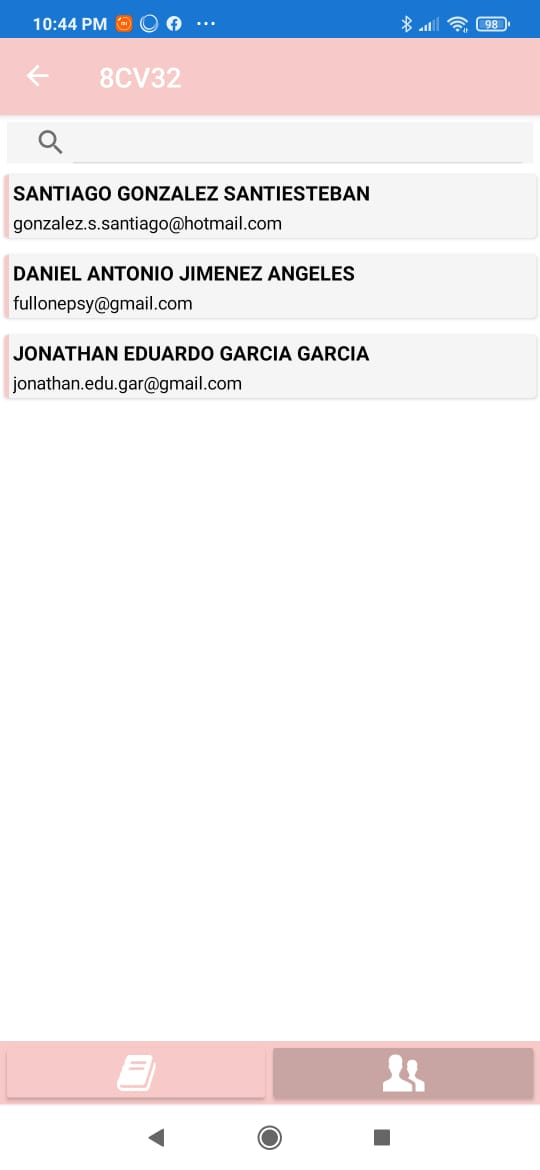
\includegraphics[width=.4\linewidth]{Imagenes/SOE15.jpeg}
        \caption{Al seleccionar una materia podemos\\ ver a los alumnos pertenecientes al grupo.}
    \end{minipage}%% 
    \vspace{1cm}
    \begin{minipage}[b]{0.49\linewidth}
        \centering
        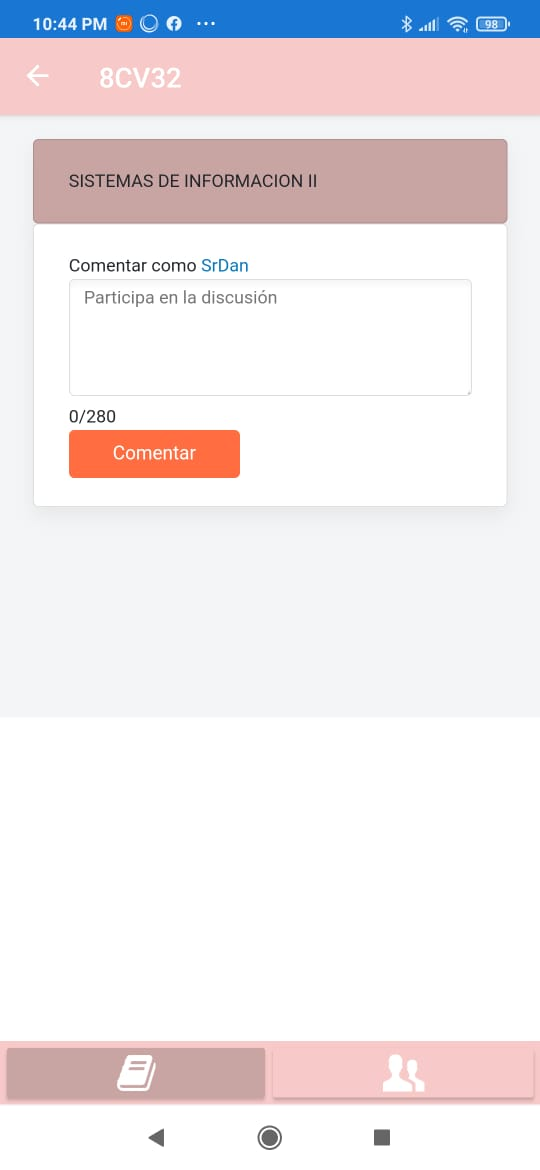
\includegraphics[width=.4\linewidth]{Imagenes/SOE16.jpeg}
        \caption{La sección de comunidad permite a los alumnos pertenecientes a alguna de las clases publicar reseñas y comentarios que podrán visualizar otros alumnos pertenecientes al grupo.}
    \end{minipage}
    \vspace{1cm}
\end{figure}

\newpage

\section{Conclusión}
\justify

El presente proyecto de inicio a fin implicó retos importantes de ellos podemos
destacar el aprendizaje para aprovisionar dinamicamente los servicios en AWS,
la recopilación de los metadatos de cada ejecución, el desarrollo de la
aplicación web para presentar la información. Esta aplicación resuelve las
necesidades que fueron identificadas durante la etapa de investigación del
desarrollo. Durante la etapa de pruebas y puesta a disposición de los pilotos
se observó una aceptación positiva por parte de los usuarios y su
retroalimentación confirma que esta aplicación es de utilidad en la realización
de pruebas de carga. Es importante destacar el apoyo que se tuvo por parte de
las materias cursadas en la Maestría en Ingeniería en Seguridad y Tecnologías
de la Información y el apoyo de los asesores que dieron las bases en el diseño
y construcción de la plataforma.

%%%%%%% Bibliografía %%%%%%%%
\nocite{*}
\addcontentsline{toc}{section}{Referencias}
\bibliographystyle{bst/IEEEtran.bst}
\bibliography{bib/IEEEreferencias.bib}

%%%%%%% Bibliografía %%%%%%%%   

\section{Anexos}
\begin{itemize}
    \item \href{https://drive.google.com/file/d/1LhLRHHiWVeEFRqgwnUttkpgct9kEACTq/view?usp=sharing} {Diseño Pantalla de tareas,  16 jun 2021}

          \par\vspace{\baselineskip}

\end{itemize}

\end{document}
